\documentclass[times, utf8, zavrsni, numeric]{fer}
\usepackage{booktabs}
\usepackage{listings}

\begin{document}

% TODO: Navedite broj rada.
\thesisnumber{5979}

% TODO: Navedite naslov rada.
\title{Sustav za dostavu hrane}

% TODO: Navedite vaše ime i prezime.
\author{Kristijan Vrbanc}

\maketitle

% Ispis stranice s napomenom o umetanju izvornika rada. Uklonite naredbu \izvornik ako želite izbaciti tu stranicu.
\izvornik

% Dodavanje zahvale ili prazne stranice. Ako ne želite dodati zahvalu, naredbu ostavite radi prazne stranice.
\zahvala{}

\tableofcontents

\chapter{Uvod}
Web aplikacije su programska rješenja kojima se pristupa putem internet preglednika. Vrtoglavi porast njihovog razvoja započeo je globalnim širenjem interneta. Danas gotovo svaka osoba ima pristup internetu, sa jednog ili više uređaja, stoga web aplikacije postaju dostupne sa bilo kojeg mjesta. 

Neovisnost o pristupu osnovna je karakteristika web aplikacija. Svi korisnici pristupaju aplikaciji na isti način, kao i ostalim web stranicama, putem internet preglednika. Također, web aplikacija je dinamična. Sadržaj se jednostavno dodaje i uklanja. Bilo koja promjena u aplikaciji odmah je vidljiva svim korisnicima. Pomoću web aplikacije moguće je ostvariti dvosmjernu komunikaciju sa korisnicima, stoga se mnoga poslovanja unaprijeđuju web aplikacijom.

Postoji velik raspon tehnologija za razvoj web aplikacija. Te tehnologije se uglavnom dijele u dva dijela, klijentske tehnologije \engl{client-side technologies} i poslužiteljske tehnologije \engl{server-side technologies}. Klijentske tehnologije služe za definiranje sučelja prema korisniku, svega što korisnik vidi i sa čime može imati interakciju. Primjeri takvih tehnologija su HTML, CSS te JavaScript. Poslužiteljske tehnologije služe za obradu podataka generiranih od strane korisnika. Primjeri takvih tehnologija su Java, Ruby, PHP, .Net.

Izrada web aplikacija je zahtjevan proces, a služi za što bolju prezentaciju na internetu. Primjeri web aplikacija su pretraživači, aplikacije za kupnju, igranje, različiti portali, email aplikacije.\\

Sustav za dotavu hrane je internet trgovina gdje korisnici na lak i intuitivan način naručuju željenu hranu. Također, sustav omogućava dostavu hrane na odabranu lokaciju. Iako današnji ubrzani način života ostavlja vrlo malo vremena za pripremu kvalitetne i ukusne hrane, korištenjem sustava moguće je poboljšati kvalitetu života uz što veću uštedu slobodnog vremena te kvalitetniju prehranu.
%------------------------------------------------------------------------------------------------------------------------------------------
\chapter{Razrada teme}
Sustav za dostavu hrane je web aplikacija arhitekture slične današnjim internet trgovinama. Prije svega, aplikacija služi za pregled jelovnika i narudžbu hrane. Od aplikacije se stoga zahtjevaju funkcionalnosti poput dodavanja restorana u sustav zajedno sa njihovim jelovnicima, kao i pregled restorana i jelovnika te mogućnost narudžbe. Također, aplikacija omogućava dostavu na željenu lokaciju, što proširuje popis traženih funkcionalnosti. Potrebno je korisnicima omogućiti unos željene lokacije. Također, potrebno je definiranje dostavljača hrane pojedinih restorana. Dostavljačima je potrebno pružiti zaseban pogled na sustav, gdje im se pruža uvid u narudžbe restorana te omogućuje preuzimanje dostava. Pritom im se pruža skup podataka potrebnih za dostavu hrane. 

Sustav podržava četiri tipa korisnika. Pogledi korisnika se razlikuju ovisno o njihovoj ulozi u sustavu. Njihova uloga također određuje prava korisnika u sustavu.

Kako bi se ostvarila takva funkcija sustava, potrebno je definirati tipove korisnika, bazu podataka te funkcionalnost same aplikacije. Također, potrebno je odabrati tehnologije za razvoj same aplikacije.  
%------------------------------------------------------------------------------------------------------------------------------------------
\section{Tipovi korisnika}
Aplikacija podržava sljedeća četiri tipa korisnika: naprijavljeni korisnik, prijavljeni korisnik sa ulogom kupca, prijavljeni korisnik sa ulogom vlasnika restorana te prijavljeni korisnik sa ulogom dostavljača hrane. Svaki tip korisnika ima prava i ograničenja određena za njega.
%------------------------------------------------------------------------------------------------------------------------------------------
\subsection{Neprijavljeni korisnik}
Neprijavljeni korisnik ima ograničena prava u sustavu. Omogućena mu je prijava u sustav ukoliko posjeduje korisnički račun ili izrada novog korisničkog računa ukoliko ga ne posjeduje. Također, neprijavljenom korisniku omogućen je pregled svih restorana sustava kao i njihovih jelovnika, ali uz nemogućnost narudžbe hrane.
%------------------------------------------------------------------------------------------------------------------------------------------
\subsection{Prijavljeni korisnik sa ulogom kupca}
Prijavljenom korisniku sa ulogom kupca, kao i neprijavljenom korisniku, omogućen je pregled svih restorana sustava i njihovih jelovnika. Glavna razika između ta dva korisnika sustava je mogućnost narudžbe. Kupcu je omogućena narudžba hrane. Prilikom narudžbe kupac ima mogućnost odabira lokacije dostave.
%------------------------------------------------------------------------------------------------------------------------------------------
\subsection{Prijavljeni korisnik sa ulogom vlasnika restorana}
Prijavljenom korisniku sa ulogom vlasnika restorana omogućeno je dodavanje restorana u sustav. Prilikom dodavanja restorana u sustav pruža osnovne podatke o restoranu (naziv, radno vrijeme, opis\ldots) kao i njegovu lokaciju. Također, omogućeno mu je definiranje jelovnika pojedinog restorana. Za pojedini restoran, omogućeno mu je dodavanje dostavljača hrane.
%------------------------------------------------------------------------------------------------------------------------------------------
\subsection{Prijavljeni korisnik sa ulogom dostavljača hrane}
Prijavljenom korisniku sa ulogom dostavljača hrane omogućen je pregled svih narudžba restorana za kojeg je nadležan. Omogućeno mu je preuzimanje dostave pojedine narudžbe pri čemu na uvid dobiva sve podatke potrebne za dostavu (popis naručenih jela i njihova količina, kontakt broj osobe koja je postavila narudžbu, smjernice\ldots).  
%------------------------------------------------------------------------------------------------------------------------------------------
\subsection{Dijagram obrazaca uporabe \engl{Use Case Diagram}}
Obrasci uporabe predstavljaju tehniku preuzetu iz UML \engl{Unified Modeling Language} standarda. UML je normirani jezik opće namjene koji se koristi za modeliranje računalnih sustava temeljenih na objektno-orijentiranoj paradigmi. Dijagram obrazaca uporabe koristi se kako bi se prikazalo ponašanje sustava, dijelova sustava ili konkretnog razreda na način vidljiv korisniku sustava \cite{UMLdijag64:online}. Slika 2.1  prikazuje  dijagram obrazaca uporabe za sva četiri tipa korisnika.
\begin{figure}[htb]
\centering
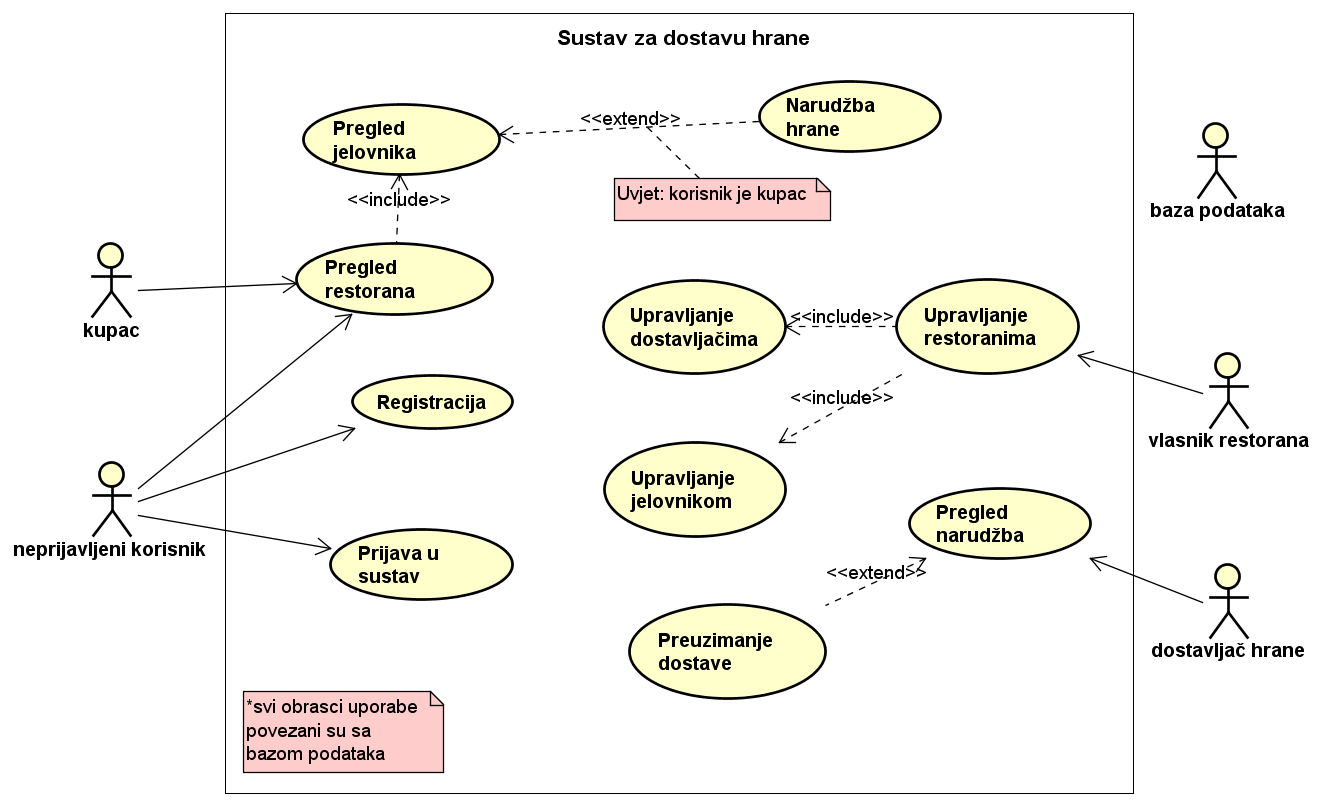
\includegraphics[height=9.0cm]{fds-useCase.png}
\caption{Dijagram obrazaca uporabe sustava}
\label{fig:use-case}
\end{figure}
%--------------------------------------------------------------------------------------------------------------------------------------------------------
\section{Korištene tehnologije}
Pri izradi aplikacije korištene su razne klijentske i poslužiteljske tehnologije. Klijentske tehnologije uključuju HTML, CSS, JavaScript te Bootsptrap. Poslužiteljske tehnologije uključuju Thymeleaf, radni okvir Spring te upitni jezik SQL.
%--------------------------------------------------------------------------------------------------------------------------------------------------------
\subsection{HTML}
Internet stranice sastoje se od različitih tipova sadržaja poput teksta, grafike, obrazaca, audio i video zapisa. Svaka internet stranica je različita, te njen izgled i funkcija ovise o tome kako je pisan kôd. Ono što internet stranice imaju zajedničko je sintaksa programiranja HTML.

HTML \engl{HyperText Markup Language} je standardni jezik za stvaranje online i offline hipertekstualnih dokumenata. HTML se kao jezik za označavanje \engl{markup language} koristi za stvaranje logičke strukture dokumenta. Označavanje se vrši korištenjem oznaka \engl{tag} kojima se stvaraju, povezuju i strukturiraju elementi HTML dokumenta. Oznake određuju način na koji će Internet preglednik prikazati tekst koji slijedi nakon oznake. HTML datoteke imaju ekstenziju \emph{.html} ili \emph{.htm}, a mogu se stvarati bilo kojim uređivačem teksta.

HTML se sastoji od elemenata i atributa. Elementi identificiraju različite dijelove HTML stranice korištenjem oznaka, a atributi daju informacije o instanci elementa. Elementi se sastoje od oznaka i sadržaja koji se nalazi unutar tih oznaka. Oznake obično dolaze u paru gdje prva oznaka započinje element, a druga ga završava. Pišu se u obliku \emph{<oznaka></oznaka>}. Sav sadržaj elementa se nalazi unutar tih oznaka, a dopušteno je i gniježđenje elemenata. Sav sadržaj koji se nalazi unutar oznaka će biti prikazan na stranici, dok se oznake koriste kao instrukcije internet pregledniku o oblikovanju tog sadržaja. Postoje elementi koji se sastoje samo od jedne oznake. Oznaka se piše u obliku \emph{<oznaka/>}. Takvi elementi zovu se prazni elementi.

HTML dokumenti sastoje se od zaglavlja i tijela dokumenta. Prva oznaka dokumenta je oznaka \emph{<html>} koja govori internet pregledniku da slijedi početak HTML dokumenta. Zadnja oznaka dokumenta je  \emph{</html>} koja označuje kraj. Zaglavlje dokumenta nalazi se unutar oznaka  \emph{<head></head>}. Sadržaj zaglavlja ne prikazuje se izravno unutar pretraživača, već služi za postavljanje elemenata koji se ne prikazuju izravno unutar pretraživača, ali mogu imati utjecaja na prikaz i ponašanje dokumenta. Tijelo dokumenta je sadržaj koji se nalazi između oznaka \emph{<body></body>}. Sadržaj koji se nalazi u tijelu dokumenta bit će vidljiv pri prikazu stranice. Slika 2.2 prikazuje primjer jednostavnog HTML dokumenta.
\begin{figure}[htb]
\centering

\includegraphics[height=3cm]{basichtml.png}
\caption{Primjer jednostavnog HTML koda}
\label{fig:basichtml}
\end{figure}
%--------------------------------------------------------------------------------------------------------------------------------------------------------
\subsection{CSS}
CSS \engl{Cascading Style Sheets}, odnosno kaskadni stilovi, mehanizam su za oblikovanje izgleda dokumenta pisanih u jezicima za označavanje (HTML, XML\ldots). CSS je dizajniran kako bi omogućio razdvajanje logičke strukture dokumenta od njegovog dizajna. Pomoću CSS-a definiraju se pravila u stilskom obrascu koji određuje izgled sadržaja opisanog određenim HTML kodom i povezuju se stilska pravila i HTML kod.  HTML kôd postaje pregledniji i manji što znači da ga je puno lakše kontrolirati, a također je moguće jednostavnom promjenom parametara promijeniti izgled stranice.

Stilski obrasci sastoje se od stilskih pravila. Svako stilsko pravilo sastoji se od selektora i deklaracije. Selektor određuje element na koji se stilsko pravilo odnosi, a deklaracija određuje izgled sadržaja opisan CSS-om. Stilsko pravilo piše se u obliku \emph{selektor\{deklaracija;\}}. Deklaracija se sastoji od svojstva \engl{property} i vrijednosti \engl{value}. Svojstva su aspekti prikaza sadržaja (boja, veličina fonta\ldots), a vrijednosti određuju iznose tih svojstva. Svojstvo se od vrijednosti odvaja dvotočjem, a svaka deklaracija završava sa točkom-zarez: \emph{selektor\{svojstvo:vrijednost;\}}. 

CSS kôd se u HTML dokument može uključitii na više načina. Kôd je moguće postaviti unutar zaglavlja dokumenta između oznaka \emph{<style></style>}. Tako postavljen kôd vrijedi na cijelom HTML dokumentu. Ukoliko se kôd zapiše unutar oznake HTML elementa, vrijedit će samo unutar tog elementa. CSS kôd također može biti zapisan u zasebnoj datoteci što omogućuje korištenje istih stilova na više različitih dokumenata. Slika 2.3 prikazuje primjer CSS koda koji postavlja boju, vrstu te veličinu fonta zaglavlja HTML dokumenta.
\begin{figure}[htb]
\centering

\includegraphics[height=2.5cm]{css-example.png}
\caption{Primjer CSS koda}
\label{fig:basicCss}
\end{figure}
%--------------------------------------------------------------------------------------------------------------------------------------------------------
\subsection{JavaScript}
JavaScript je dinamički programski jezik koji, ukoliko se ugradi u HTML dokument, može pružiti dinamičku interakciju na stranici. Dinamički programski jezici su programski jezici u kojima se operacije koje se inače izvrše u vrijeme prevođenja mogu izvršiti tijekom izvođenja\cite{Dynamicp76:online}. Jezik JavaScript podržan je od strane svih internetskih preglednika.

Izvorni kod pisan jezikom JavaScript ugrađuje se u tijelo HTML dokumenta unutar oznaka \emph{<script></script>}. JavaScript omogućava izradu interaktivnih web stranica zbog mogučnosti  pristupa i izmjene sadržaja i oznaka koje se koriste u HTML dokumentu za vrijeme njegovog prikazivanja. Slika 2.4 prikazuje jednostavni JavaScript kôd ugrađen u HTML dokument. Prilikom učitavanja dokumenta, u njegovo tijelo upisuje se tekst.
\begin{figure}[htb]
\centering
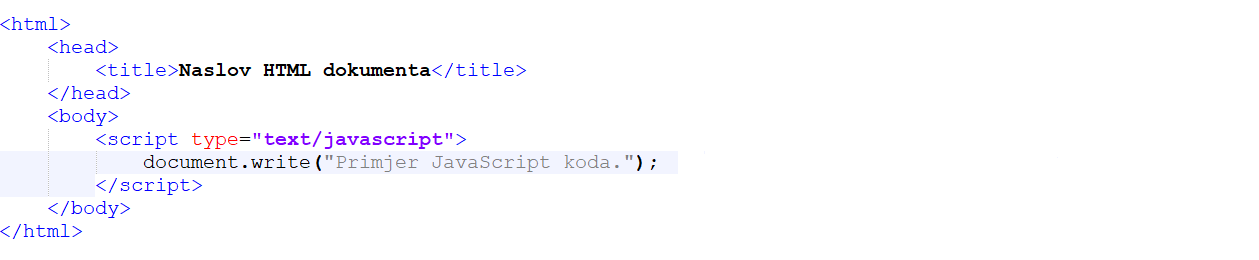
\includegraphics[height=4cm]{js-example.png}
\caption{Primjer JavaScript koda}
\label{fig:basicJs}
\end{figure}
%--------------------------------------------------------------------------------------------------------------------------------------------------------
\subsubsection{Maps JavaScript API}
JavaScript API \engl{Application Programming Interface} za Google Karte \engl{Google Maps} omogućuje prilagođavanje karata vlastitim sadržajem i slikama u svrhu prikaza na web stranicama i mobilnim uređajima. JavaScript API za Karte sadrži četiri osnovna tipa karata (cestovna karta \engl{roadmap}, satelit \engl{satellite}, hibrid \engl{hybrid} i teren \engl{terrain}) koje se mogu mijenjati korištenjem slojeva i stilova, kontrola i događaja te raznih usluga i knjižnica\cite{Overview86:online}. Slika 3.4 prikazuje kôd web stranice koja prikazuje kartu sa središtem u Zagrebu.
\begin{figure}[htb]
\centering
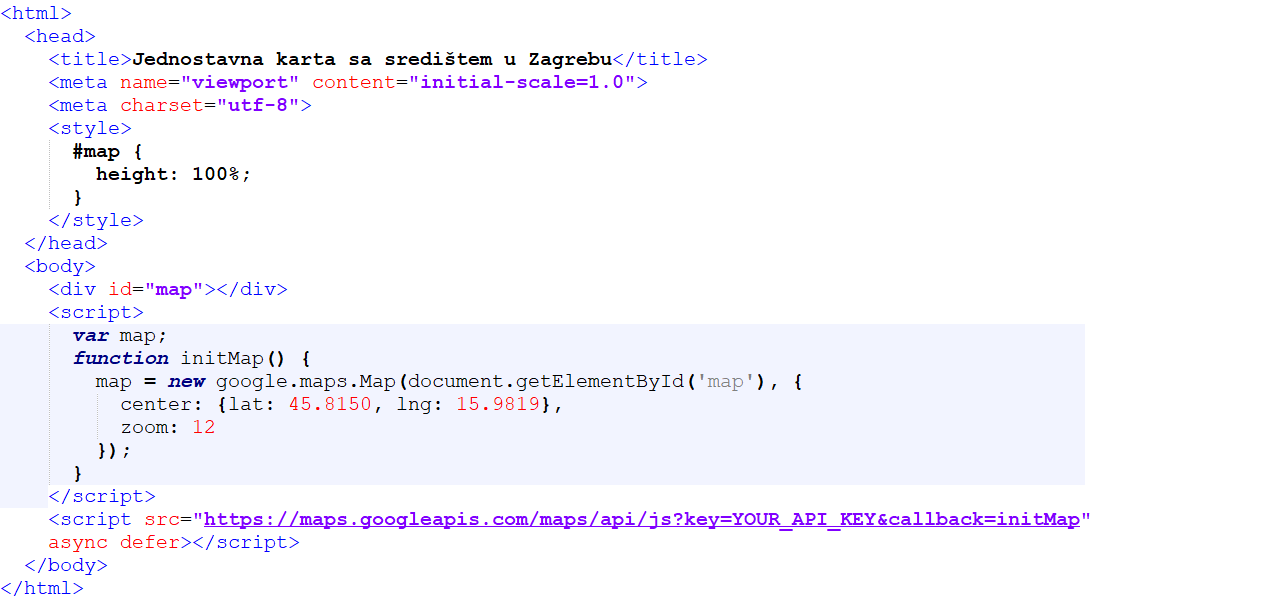
\includegraphics[height=8cm]{maps-js-api.png}
\caption{Kod web stranice koja prikazuje kartu sa središtem u Zagrebu}
\label{fig:mapsJs}
\end{figure}
%--------------------------------------------------------------------------------------------------------------------------------------------------------
\subsubsection{Geocoding API}
Geocoding API je usluga koja pruža geokodiranje i obrnuto geokodiranje adresa. Geokodiranje je postupak pretvorbe adresa u zemljopisne koordinate (kao što su zemljopisna širina i dužina) koje se mogu koristiti za postavljanje oznaka na kartu ili postavljanje karte\cite{GetStart0:online}. Obrnuto geokodiranje je postupak pretvorba zemljopisnih koordinata u adrese.

Pristup usluzi Geocoding vrši se preko HTTP sučelja. Slanjem HTTP zahtjeva standardiziranog oblika dobiva se odgovor od poslužitelja. U kontekstu geokodiranja, odgovor sadrži zemljopisnu širinu i dužinu adrese za koju je podnijet zahtjev. U kontekstu obrnutog geokodiranja, odgovor sadrži formatiranu adresu koja se nalazi na određenoj zemljopisnoj širini i dužini. Odgovor je formata JSON \engl{JavaScript Object Notation}, stoga se vrlo lako obrađuje korištenjem jezika JavaScript. Slika 3.5 prikazuje primjer HTTP zahtjeva za geokodiranje adrese \emph{Unska 3, Zagreb}.
\begin{figure}[htb]
\centering

\includegraphics[height=0.48cm]{geocoding-api.png}
\caption{Prikaz HTTP zahtjeva za geokodiranjem adrese}
\label{fig:geocodeJs}
\end{figure}
%----------------------------------------------------------------------------------------------------------------------------------------------------------
\subsubsection{Directions API}
Directions API je usluga koja računa smjernice između lokacija. Smjernice se mogu tražiti za nekoliko načina prijevoza, uključujući javni prijevoz, vožnju automobilom, hodanje ili vožnju biciklom\cite{GetStart97:online}.

Pristup usluzi Directions vrši se preko HTTP sučelja. Zahtjev je standardiziranog oblika, konstruiran kao URL koristeči adrese ili zemljopisne širine i dužine za identifikaciju lokacija. Korištenjem jezika JavaScript može se postići dinamička promjena zahtjeva. Slika 3.6 prikazuje primjer HTTP zahtjeva za smjernice između lokacija \emph{Unska 3} i \emph{Ulica grada Vukovara 114}.
\begin{figure}[htb]
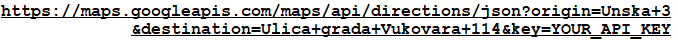
\includegraphics[height=1cm]{directions-api.png}
\caption{Prikaz HTTP zahtjeva za smjernice}
\label{fig:directionsJs}
\end{figure}
%----------------------------------------------------------------------------------------------------------------------------------------------------------
\subsection{Bootstrap}
Bootstrap je jedan od najpopularnijih HTML, CSS  i JavaScript razvojnih okvira razvijen od strane Twittera, čija je svrha razvoj prilagodljivih web aplikacija. Sastoji se od niza predloška \engl{templates} razvijenih tehnologijama HTML i CSS, za uobičajene HTML elemente korisničkog sučelja poput tablica, formulara, navigacijskih traka, padajućih izbornika\ldots Bootstrap je moguće koristiti uz bilo koju poslužiteljsku tehnologiju.

Korištenje razvojnog okvira Bootstrap nosi mnoge prednosti. Web stranice koje koriste Bootstrap automatski se prilagođuju različitim veličinama ekrana, stoga mijenjaju svoj dizajn ovisno o uređaju na kojem se prikazuju. Korištenje Bootstrapa u razvoju aplikacije može uštedjeti mnogo vremena. Bootstrap nudi gotove blokove HTML, CSS i JavaScript koda koji se mogu koristiti i prilagoditi potrebama aplikacije.  

Kako bi se koristio Bootstrap unutar web stanice potrebno je povezati stranicu sa CSS i JavaScript datotekama razvojnog okvira. Povezivanje sa CSS datotekama izvodi se u zaglavlju HTML dokumenta unutar praznog elementa \emph{<link>} dok se povezivanje sa JavaScript datotekama izvodi u tijelu HTML dokumenta unutar oznaka \emph{<script></script>}. Slika 2.8 prikazuje kôd jednostavne web stranice koja koristi razvojni okvir Bootstrap.
\begin{figure}[htb]
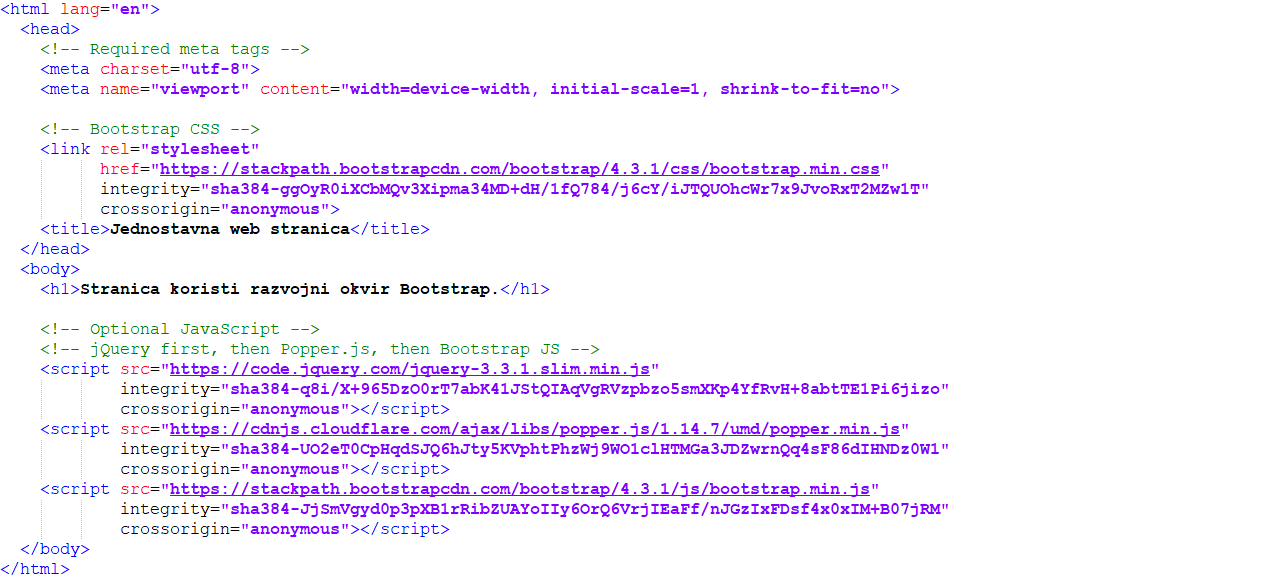
\includegraphics[height=9cm]{basic-bootstrap.png}
\caption{Jednostavna web stranica koja koristi razvojni okvir Bootstrap\cite{Introduc43:online}}
\label{fig:basicBs}
\end{figure}

%----------------------------------------------------------------------------------------------------------------------------------------------------------
\subsection{Razvojni okvir Spring}
Razvojni okvir Spring olakšava stvaranje aplikacija koristeći platformu Java EE \engl{Java Enterprise Edition}. Platforma Java EE pruža API i  okruženje izvođenja potrebnih za razvoj velikih, višeslojnih, skalabilnih, pouzdanih i sigurnih mrežnih aplikacija\cite{Differen48:online}. Uz programski jezik Java, Spring sadrži podršku za jezike Groovy i Kotlin kao alternativne jezike na JVM \engl{Java virtual machine}.

Spring je razvojni okvir otvorenog koda. Ima veliku aktivnu zajednicu koja osigurava kontinuiranu povratnu informaciju temeljenu na raznolikim slučajevim korištenja u stvarnom svijetu\cite{SpringFr9:online}.

Razvojni okvir Spring podijeljen je u module. Aplikacije mogu odabrati koji moduli su im potrebni. U središtu su moduli jezgrenog spremnika, uključujuči i mehanizam za ubrizgavanje zavisnisti \engl{dependency injection mechanism}. Ubrizgavanje zavisnosti je naziv za prijenos odgovornosti stvaranja objekta na neki drugi objekt i izravno korištenje te stvorene ovisnosti.  Također, Spring osigurava temeljnu podršku za različite arhitekture aplikacija, uključujući slanje poruka, prijenos podataka te web.
%----------------------------------------------------------------------------------------------------------------------------------------------------------
\subsubsection{Spring Boot}
Spring Boot pruža dobru platformu za razvoj samostalnih i proizvodno spremnih aplikacija koje se mogu odmah pokrenuti. Također, omogućuje početak sa minimalnim konfiguracijama bez potrebe za čitavom konfiguracijom razvojnog okvira Spring.

Spring Boot konfigurira aplikaciju na temelju okoline, kao i onih informacija koje razvojni programer pruži. Aplikacija koja koristi Spring Boot potpuno je samostalna. Aplikaciju nije potrebno postaviti na web poslužitelj ili neko posebno okruženje kako bi se pokrenula.
%----------------------------------------------------------------------------------------------------------------------------------------------------------
\subsubsection{Spring Web MVC}
Spring MVC \engl{Model-View-Controller} okvir pruža Model-Pogled-Upravljač arhitekturu i spremne komponente koje se mogu koristiti za razvoj fleksibilnih web aplikacija. Uzorak MVC rezlutira razdvajanjem razičitih aspekata aplikacije poput ulazne logike, poslovne logike i korisničkog sučelja, dok istovremeno pruža vezu imeđu tih elemenata.

\emph{Model} objedinjuje podatke aplikacije i općenito se sastoji od objekata POJO \engl{Plain Old Java Object}. POJO je običan Java objekt nevezan nikakvim posebnim ograničenjima osim onih koja zahtijeva programski jezik Java. \emph{Pogled} je odgovoran za prikazivanje podataka modela i općenito stvara HTML izlaz koji klijentski preglednik može interpretirati. \emph{Upravljač} obrađuje korisničke zatjeve i odgovoran je za gradnju modela kojeg prosljeđuje pogledu za stvaranje prikaza. Slika 2.9 prikazuje upravljač zahtjeva potvrde korisničkog računa.
\begin{figure}[htb]
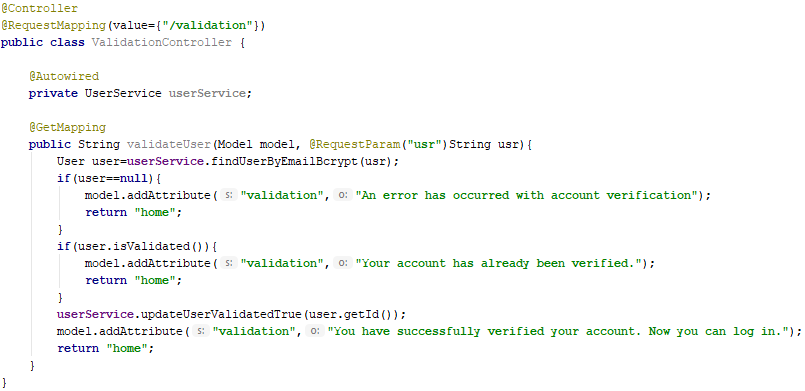
\includegraphics[height=7.5cm]{validation-controller.png}
\caption{Upravljač zahtjeva potvrde korisničkog računa}
\label{fig:controller}
\end{figure}
%----------------------------------------------------------------------------------------------------------------------------------------------------------
\subsubsection{Spring Security}
Spring Security je snažan i vrlo prilagodljiv okvir za provjeru autentičnosti i pristupa. To je modul ravojnog okvira Spring usmjeren na pružanje i provjeru autentičnosti i autorizacije za Java aplikacije. Snaga Spring Security modula nalazi se u lakoći proširenja u svrhu zadovoljenja određenih zahtjeva. Slika 2.10 prikazuje konfiguraciju modula Spring Security kako bi se svim korisnicima omogućili zahtjevi poput pregleda restorana sustava i njihovih jelovnika, a ograničili zahtjevi poput pregleda košarice ili pregleda narudžba samo na korisnike sa određenom ulogom u sustavu. 
\begin{figure}[htb]
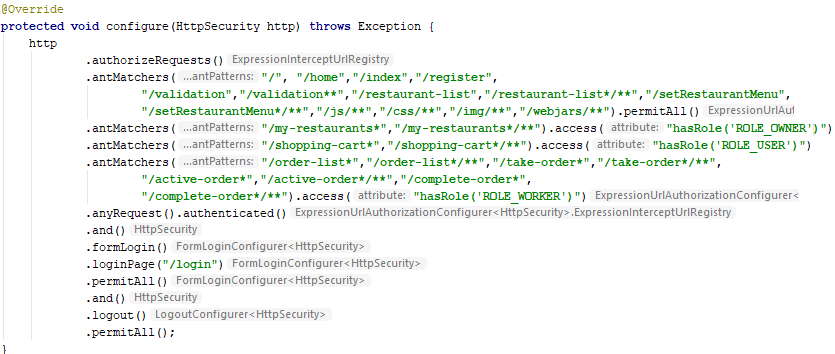
\includegraphics[height=7.0cm]{security.png}
\caption{Konfiguracija modula Spring Security}
\label{fig:security}
\end{figure}
%----------------------------------------------------------------------------------------------------------------------------------------------------------
\subsubsection{Spring Data JPA}
Spring Data JPA \engl{Java persistance API}, dio veće Spring Data obitelji, olakšava implementiranje spremišta \engl{repositories} baziranih na JPA. Ovaj se modul bavi podrškom JPA baziranom sloju za pristup podacima.

Implementacija sloja za pristup podacima je već dulje vrijeme neefikasna, popraćena sa puno programskog koda. Veliku količinu koda potrebno je napisati kako bi se izvršili jednostavni upiti nad bazom podataka. Spring Data JPA značajno poboljšava implementaciju slojeva za pristup podacima, smanjenjem potrebnog koda. Sve što je potrebno je definirati sučelja spremišta, uključujući prilagođene metode pretrage podataka, a Spring omogućava automatsku implementaciju. Slika 2.11 prikazuje implementaciju spremišta za pohranu korisnika sustava. Šest nevedenih metoda pretrage prilagođene su potrebama aplikacije.
\begin{figure}[htb]
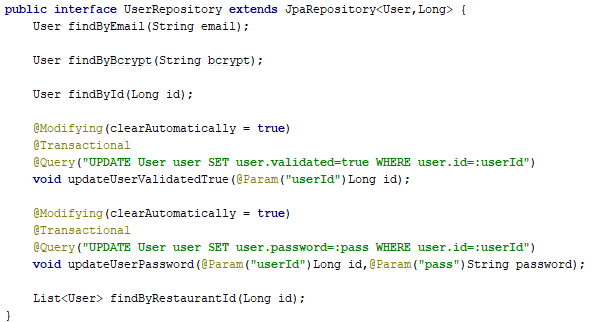
\includegraphics[height=7.0cm]{jpa.png}
\caption{Implementacija spremišta za pohranu korisnika sustava}
\label{fig:jpa}
\end{figure}
%----------------------------------------------------------------------------------------------------------------------------------------------------------
\subsection{Thymeleaf}
Thymeleaf je Java knjižnica. To je XML / XHTML / HTML5 obrađivač predloška \engl{template engine} koji može primjeniti skup transformacija na datoteke predloška kako bi se prikazali podaci stvoreni aplikacijom. Thymeleaf je najprikaldniji za obradu XHTML / HTML5 datoteka u web aplikacijama, ali može obraditi i bilo koju XML datoteku na webu ili samostalno.

Primarni cilj tehnologije Thymeleaf je pružiti elegantan i strukturiran način izrade predložaka. Kako bi se to postiglo, Thymeleaf je temeljen na XML oznakama i atributima koji određuju izvođenje unaprijed definirane logike nad modelom DOM \engl{Document Object Model}. Arhitektura tehnologije Thymeleaf omogućuje brzu obradu predloška, oslanjajući se na predmemoriranje obrađenih datoteka kako bi se koristila što manja količina ulazno izlaznih operacija.

Razvojni uzorak MVC je metoda za odvajanje problema unutar web aplikacije. Logika aplikacije odvojena je od tehnologija za prikaz informacija korisniku. Model prenosi podatke između logike aplikacije i sloja prikaza. Unutar aplikacije, sloj pregleda može koristiti jednu ili više različitih tehnologija za obradu pogleda. Web aplikacije razvijene u razvojnom okviru Spring podržavaju različite opcije prikaza koji se često nazivaju prikazni predlošci \engl{view templates}. Te se tehnologije nazivaju predlošci jer pružaju jezik za označavanje koji omogućava izlaganje atributa modela unutar prikaza tijekom prikazivanja na strani klijenta.

Slika 2.12 prikazuje dio HTML koda obogaćenog XML oznakama tehnologije Thymeleaf. Oznake sadrže prefiks \emph{th} i dvotočje. Prikazani kod služi za prikaz podataka o korisničkim računima dostavljača pojedinog restorana. Prikaz se ostvaruje prolaskom po elementima atributa modela naziva  \emph{workerList}, koji je zapravo lista korisnika. Prikazuju se njihove email adrese sa pripadnim lozinkama.
\begin{figure}[htb]
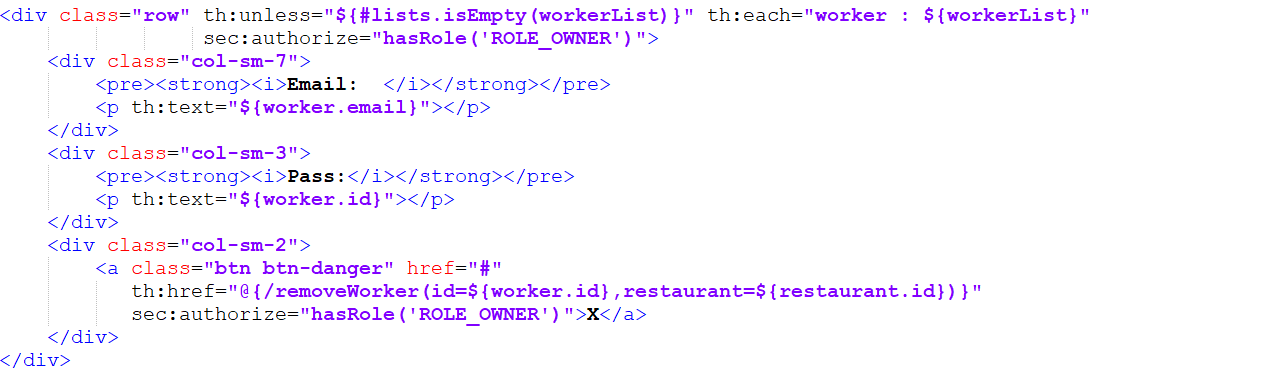
\includegraphics[height=5.0cm]{thymeleaf.png}
\caption{Prikaz podataka o korisničkim računima dostavljača}
\label{fig:thymeleaf}
\end{figure}
%----------------------------------------------------------------------------------------------------------------------------------------------------------
\subsection{SQL}
SQL \engl{Structured Query Language} je standardni računalni jezik za upravljanje relacijskim bazama podataka i manipulaciju podacima. Korištenjem jezika SQL nad bazom podataka mogu se provesti razne operacije poput umetanja podataka u postojeće tablice baze podataka i brisana podataka. Uz to, može se mijenjati sama struktura baze podataka stvaranjem, mijenjanjem i brisanjem tablica i drugih objekata baze podataka.

SQL kod podijeljen je u četiri glavne kategorije: upiti, dio jezika za manipulaciju podacima naziva DML \engl{Data Manipulation Language}, dio jezika za definiranje podataka naziva DDL \engl{Data Definition Language} te dio jezika za upravljanje podacima naziva DCL \engl{Data Control Language}.

\emph{Upiti} se izvode pomoću SELECT izraza, koji je nadalje podijeljena na klauzule, uključujući SELECT, FROM, WHERE i ORDER BY.

\emph{DML} se koristi za dodavanje, promjenu ili brisanje podataka. Zapravo je podskup izraza SELECT i sastoji se od INSERT, DELETE i UPDATE izraza, kao i kontrolnih izraza poput BEGIN TRANSACTION, SAVEPOINT, COMMIT i ROLLBACK.

\emph{DDL} se koristi za upravljanje strukturama baze podataka. Sasatoji se od izraza poput CREATE, ALTER, TRUNCATE i DROP.

\emph{DCL} se koristi za dodjeljivanje i opoziv prava i dozvola nad bazama podataka. Glavni izrazi tog skupa su GRANT i REVOKE.
%----------------------------------------------------------------------------------------------------------------------------------------------------------
\section{Baza podataka}
Baza podataka je skup zapisa pohranjenih u računalu na sustavan način. Svaki zapis uobičajeno se sastoji od skupa elemenata podataka. Računalni program korišten za upravljanje i ispitivanje baze podataka naziva se sustav upravljanja bazom podataka.

Aplikacija koristi PostgreSQL sustav upravljanja bazom podataka. PostgreSQL je objektno-relacijski sustav upravljanja bazom podataka koji koristi i proširuje sintaksu SQL jezika. PostgreSQL radi na svim većim operacijskim sustavima, a od 2001. godine je kompatibilan sa svojstvima ACID ( atomarnost \engl{atomicity}, dosljednost \engl{consistency}, izoliranost \engl{isolation}, trajnost \engl{durability})\cite{PostgreS70:online}.

Slika 2.13 prikazuje dijagram baze podataka, a u nastavku slijedi kratki opis pojedine tablice.
\begin{figure}[htb]
\centering
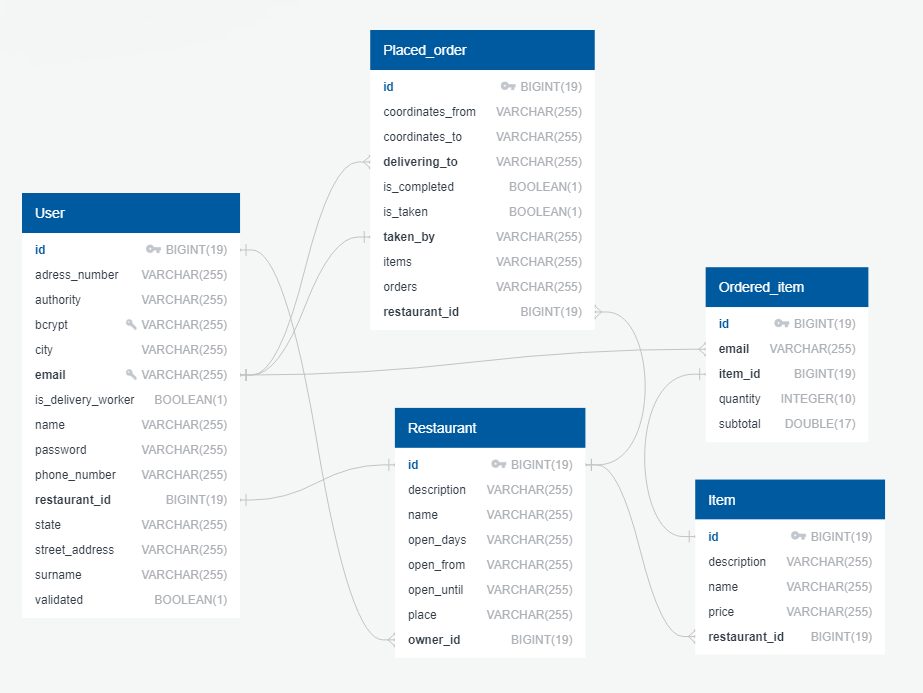
\includegraphics[height=11cm]{database.png}
\caption{Dijagram baze podataka}
\label{fig:db}
\end{figure}
%----------------------------------------------------------------------------------------------------------------------------------------------------------
\subsection{Tablica User}
Tablica User služi za pohranu svih registriranih korisnika. Sadrži podatke koje korisnik pruža prilikom registracije, kao i neke dodatne podatke bitne za rad aplikacije. Tablica User je centralna tablica u bazi podataka jer se na nju veže većina ostalih tablica. Primarni ključ tablice je \emph{id} koji je cjelobrojnog tipa i postavljen na automatsko povećavanje svakim uzastopnim korisnikom dodanim u bazu. Polje \emph{email} postavljeno je kao jedinstveni indeks kako bi se spriječilo registriranje više korisničkih računa putem jedne email adrese. Razlog tomu je prijava u sustav koja se vrši preko email adrese i pripadne lozinke. Polje \emph{authority} služi za definiranje uloge korisnika u sustavu. Može poprimiti vrijednosti ROLE\_OWNER (definira korisnika kao vlasnika restorana), ROLE\_USER ( definira korisnika kao kupca) te ROLE\_WORKER (definira korisnika kao dostavljača hrane). Polja \emph{bcrypt} i \emph{validated} služe za validaciju korisnika putem elektroničke pošte. Polje \emph{is\_delivery\_worker} i \emph{restaurant\_id} služe za definiranje korisnika kao dostavljača i vezu sa restoranom za kojeg je nadležan. Ostala polja sadrže osobne podatke korisnika.
%----------------------------------------------------------------------------------------------------------------------------------------------------------
\subsection{Tablica Restaurant}
Tablica Restaurant služi za pohranu svih restorana sustava. Sadrži podatke koje korisnik sustava sa ulogom vlasnika restorana pruža prilikom dodavanja restorana u sustav. Ti podaci sadrže ime i opis restorana, kao i dane u tjednu tijekom kojih je restoran otvoren sa pripadnim radnim vremenom. Primarni ključ tablice je \emph{id} koji je cjelobrojnog tipa i postavljen na automatsko povećavanje svakim uzastopnim restoranom dodanim u bazu. Polje \emph{place} sadrži geografsku lokaciju (u obliku geografske širine i dužine) koju je korisnik postavio za svoj restoran. Polje \emph{owner\_id} služi kao veza sa tablicom User koja određuje vlasnika tog restorana.
%----------------------------------------------------------------------------------------------------------------------------------------------------------
\subsection{Tablica Item}
Tablica Item služi za pohranu prehrambenih proizvoda. Sadrži podatke koje korisnik sustava sa ulogom vlasnika restorana pruža prilikom dodavanja proizvoda u sustav. Ti podaci sadrže ime i opis proizvoda kao i njegovu jediničnu cijenu. Primarni ključ tablice je \emph{id} koji je cjelobrojnog tipa i postavljen na automatsko povećavanje svakim uzastopnim proizvodom dodanim u bazu. Element \emph{restaurant\_id} služi kao veza sa tablicom Restaurant te određuje pripadnost tom restoranu.
%----------------------------------------------------------------------------------------------------------------------------------------------------------
\subsection{Tablica Ordered\_item}
Tablica Ordered\_item služi za pohranu prehrambenih proizvoda koji se nalaze u košarici pojedinog korisnika. Primarni ključ tablice je \emph{id} koji je cjelobrojnog tipa i postavljen na automatsko povećavanje svakim uzastopnim dodavanjem proizvoda u košaricu. Polje \emph{email} sadrži email adresu korisnika koji je stavio proizvod u košaricu te služi kao veza prema tablici User. Polje \emph{item\_id} služi za povezivanje sa tablicom Item te određuje naručeni proizvod. Polja \emph{quantity} i \emph{subtotal} određuju brojnost i ukupnu cijenu naručenog proizvoda.
%----------------------------------------------------------------------------------------------------------------------------------------------------------
\subsection{Tablica Placed\_order}
Tablica Placed\_order služi za pohranu narudžba sustava. Sadrži podatke koji se prosljeđuju dostavljačima hrane. Svrha ove tablice je omogućavanje naručivanja prehrambenih proizvoda iz više različitih restorana.  Primarni ključ tablice je \emph{id} koji je cjelobrojnog tipa i postavljen na automatsko povećavanje svakim uzastopnim dodavanjem narudžbe u bazu. Polja \emph{coordinates\_from} i \emph{coordinates\_to} definiraju geografsku lokaciju restorana te geografsku lokaciju koju je pružao korisnik prilikom narudžbe. Te se lokacije koriste prilikom prikaza uputa dostavljaču putem usluge Directions. Polje \emph{delivering\_to} služi kao poveznica sa tablicom User i određuje korisnika koji je podnio narudžbu. Polja \emph{is\_taken} i \emph{taken\_by} ažuriraju se prilikom preuzimanja naružbe. Svrha tih polja je onemogućavanje preuzimanja narudžbe od strane više dostavljača. Ukoliko je dostava izvršena, ažurira se vrijednost polja \emph{is\_completed}. Polje \emph{items} sadrži ključeve proivoda, dok \emph{quantities} sadrži brojnost proizvoda narudžbe. Polje \emph{restaurant\_id} služi kao poveznica sa tablicom Restaurant te određuje pripadnost pojedinom restoranu.
%----------------------------------------------------------------------------------------------------------------------------------------------------------
\section{Opis funkcionalnosti}
Sustav se sastoji od više stranica koje nude različite funkcionalnosti. Slijedi opis pojedinih stranica.
%----------------------------------------------------------------------------------------------------------------------------------------------------------
\subsection{Početna stranica}
Početna stranica korisnicima prikazuje kratki opis usluga koje aplikacija pruža. Također, pružan je pregled lokacija svih restorana sustava korištenjem usluge Google Maps. Sadržaj navigacijske trake razlikuje se ovisno o ulozi pojedninog korisnika u sustavu.

Slika 2.14 prikazuje početnu stranicu neprijavljenog korisnika. Navigacijska traka sastoji se od poveznica \emph{Home}, \emph{Login}, \emph{Register} i \emph{Restaurants}. Tim poveznicama korisnik ostvaruje tražene funkcionalnosti sustava. Pristup stranici za prijavu u sustav ostvaruje se poveznicom \emph{Login}, a pristup stranici za izradu novog korisničkog računa poveznicom \emph{Register}. Korisnik pristupa stanici za pregled svih restorana sustava poveznicom \emph{Restaurants}. Poveznica \emph{Home} korisnika prosljeđuje ponovno na početnu stranicu. 
\begin{figure}[htb]
\centering
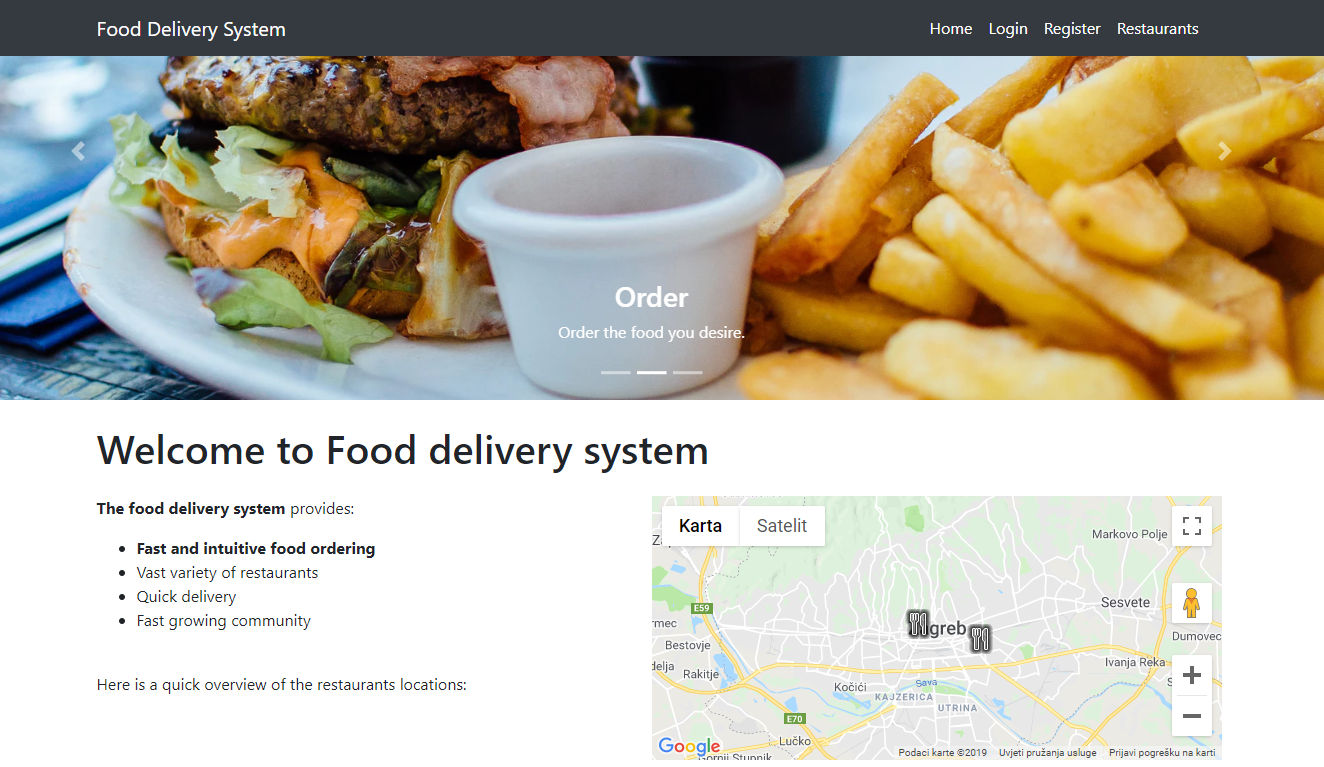
\includegraphics[height=8.5cm]{pocetna-neprijavljeni.png}
\caption{Početna stranica naprijavljenog korisnika}
\label{fig:pocNep}
\end{figure}

Navigacijska traka svih prijavljenih korisnika sadrži prikaz korisničkog imena korištenog za prijavu u sustav te mogućnost odjave iz sustava poveznicom \emph{Sign out}.

Slika 2.15 prikazuje navigacijsku traku prijavljenog korisnika sa ulogom kupca. Kao i kod neprijavljenog korisnika, traka sadrži poveznice \emph{Home} i \emph{Restaurants}. Također, kupcu je omogućena narudžba hrane stoga mu je prikazana poveznica u obliku košarice za kupnju. Putem nje, korisnik pristupa svojoj virtualnoj košarici.
\begin{figure}[htb]
\centering

\includegraphics[height=0.55cm]{pocetna-kupac.png}
\caption{Navigacijska traka prijavljenog korisnika sa ulogom kupca}
\label{fig:pocKup}
\end{figure}

Slika 2.16 prikazuje navigacijsku traku prijavljenog korisnika sa ulogom vlasnika restorana. Uz poveznicu \emph{Home}, traka vlasnika restorana sadrži i poveznicu \emph{My restaurants}. Tom poveznicom korisnik pristupa stranici sa popisom njegovih restorana te opcijom dodavanja novog.
\begin{figure}[htb]
\centering

\includegraphics[height=0.6cm]{pocetna-vlasnik.png}
\caption{Navigacijska traka prijavljenog korisnika sa ulogom vlasnika restorana}
\label{fig:pocVlas}
\end{figure}

Navigacijska traka prijavljenog korisnika sa ulogom dostavljača hrane nalazi se na slici 2.17. Kao i kod svih korisnika, traka sadrži poveznicu \emph{Home}. Također, traka sadrži poveznice \emph{Active order} i \emph{Orders}. Prisup popisu svih narudžbi restorana za kojeg je nadležan korisnik ostvaruje poveznicom \emph{Orders}. Poveznicom \emph{Active order} korisnik pristupa stranici svoje trenutno aktivne dostave.
\begin{figure}[htb]
\centering

\includegraphics[height=0.6cm]{pocetna-dostavljac.png}
\caption{Navigacijska traka prijavljenog korisnika sa ulogom dostavljača hrane}
\label{fig:pocDost}
\end{figure}
%----------------------------------------------------------------------------------------------------------------------------------------------------------
\subsection{Registracija}
Korisnik izrađuje novi korisnički račun upisujući potrebne podatke u obrazac na stranici registracije. Stranica registracije prikazana je na slici 2.18. Sva polja obrasca su obavezna. Sadrže podatke poput email adrese i lozinke koje će korisnik kasnije koristiti prilikom prijave, kao i osobne podatke poput imena i prezimena, kontakt broja te adrese prebivališta. Prilikom registracije korisnik izjavljuje koju ulogu želi poprimiti u sustavu. Izabire između uloge kupca i uloge vlasnika restorana.
\begin{figure}[htb]
\centering
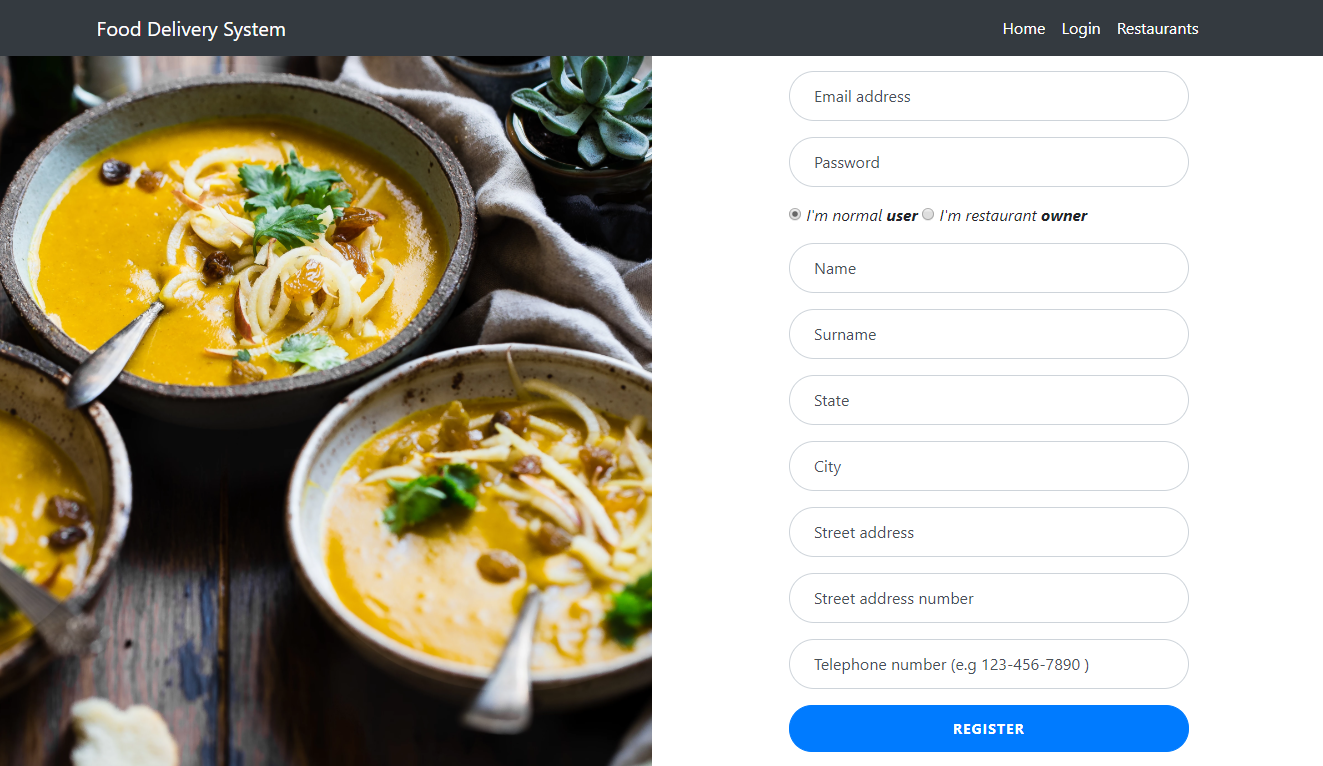
\includegraphics[height=8.0cm]{registracija.png}
\caption{Registracijska stranica}
\label{fig:regis}
\end{figure}

Nakon uspješne registracije koja iziskuje email adresu koja je jedinstvena u sustavu, na tu adresu šalje se verifikacijksa poveznica koja potvrđuje izradu korisničkog računa. Ukoliko se račun ne potvrdi, korisniku je onemogućena prijava u sustav.
%----------------------------------------------------------------------------------------------------------------------------------------------------------
\subsection{Prijava}
Korisnik se prijavljuje koristeči svoju email adresu i lozinku. Slika 2.19 prikazuje stranicu prijave. Preduvjet uspješnoj prijavi korisnika je 
posjedovanje korisničkog računa koji je verificiran putem email adrese. Ukoliko korisnik unese podatke koji se ne nalaze u sustavu ispisuju mu se odgovarajuće poruke upozorenja.
\begin{figure}[htb]
\centering
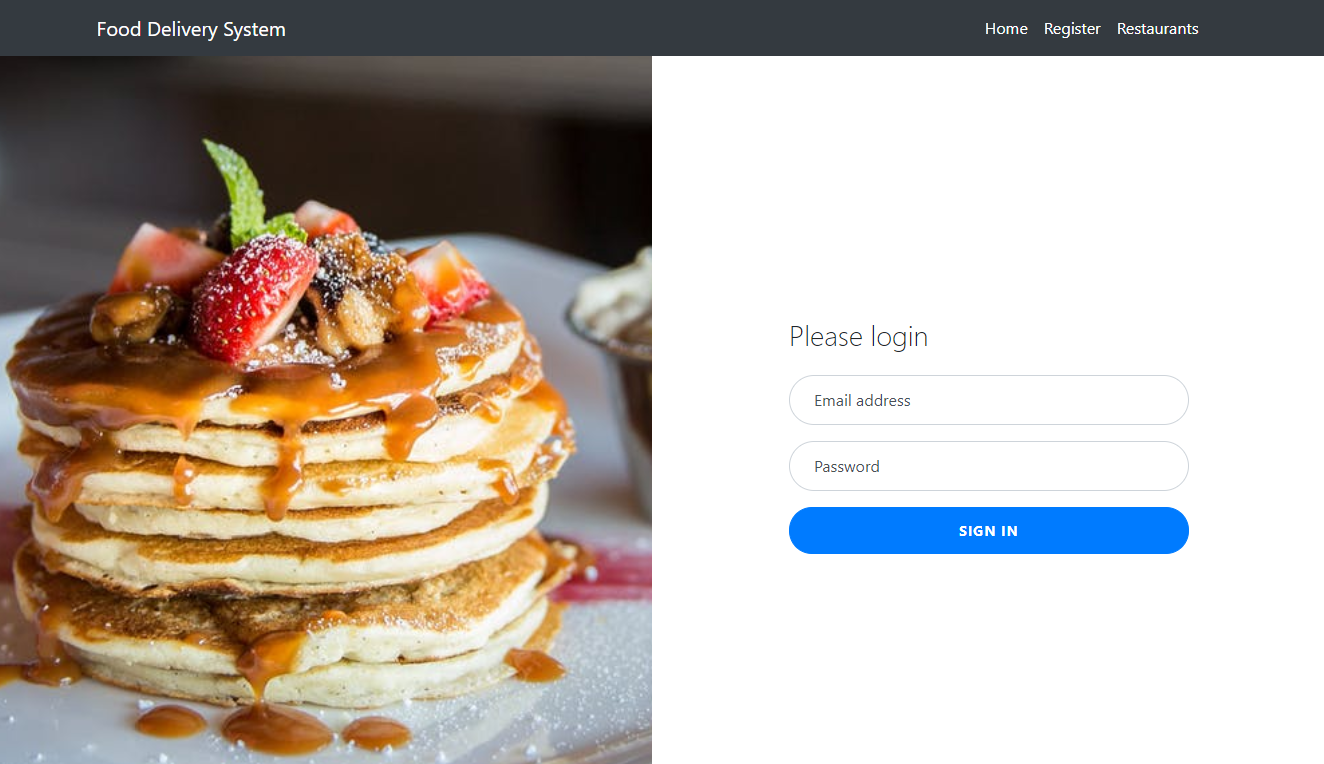
\includegraphics[height=7.8cm]{login.png}
\caption{Stranica za prijavu u sustav}
\label{fig:login}
\end{figure}
%----------------------------------------------------------------------------------------------------------------------------------------------------------
\subsection{Pregled restorana sustava}
Neprijavljeni korisnici te korisnici sa ulogom kupca u sustavu mogu pristupiti stranici za pregled svih restorana sustava koja je prikazana na slici 2.20. Stranica sadrži popis restorana sa njihovim kratkim opisima. Kratki opis sadrži naziv restorana, opis, radno vrijeme te dane u tjednu tijekom kojih je restoran otvoren za poslovanje. Također, korisnicima se prikazuje slika restorana učitana od strane vlasnika. Poveznica \emph{View menu} vodi korisnika na stranicu za pregled jelovnika restorana.
\begin{figure}[htb]
\centering
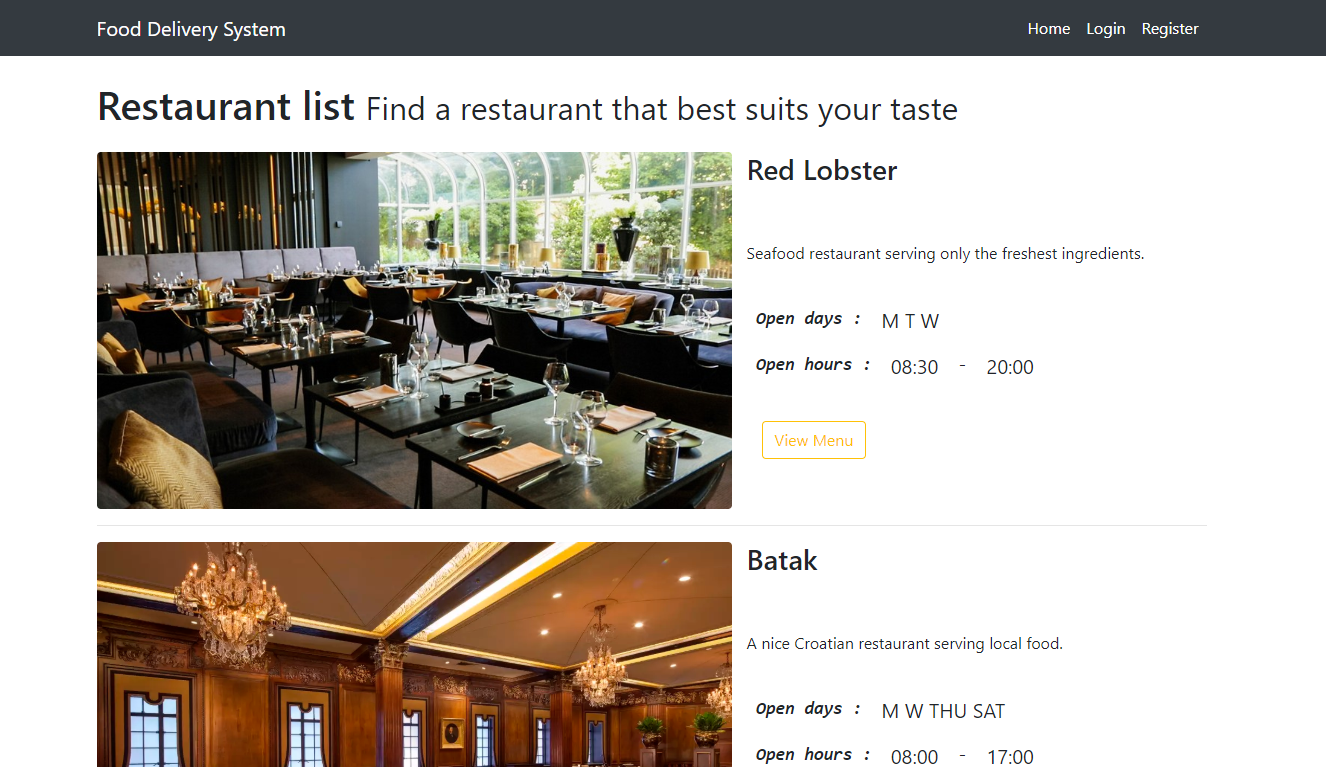
\includegraphics[height=8.5cm]{restaurants.png}
\caption{Stranica za pregled svih restorana sustava}
\label{fig:allRest}
\end{figure}
%----------------------------------------------------------------------------------------------------------------------------------------------------------
\subsection{Pregled vlastitih restorana}
Korisnicima sa ulogom vlasnika u sustavu omogućen je pregled vlastitih restorana. Stranica prikazana na slici 2.21 pruža korisniku pregled  svih restorana koje je prethodno dodao u sustav. Kao i kod pregleda restorana sustava, svaki restoran prikazan je svojim kratkim opisom i slikom. Vlasniku je također omogućeno uklanjanje restorana iz sustava korištenjem poveznice \emph{Remove} te odlazak na stranicu za pregled jelovnika putem povezince \emph{Manage restaurant}.
\begin{figure}[htb]
\centering
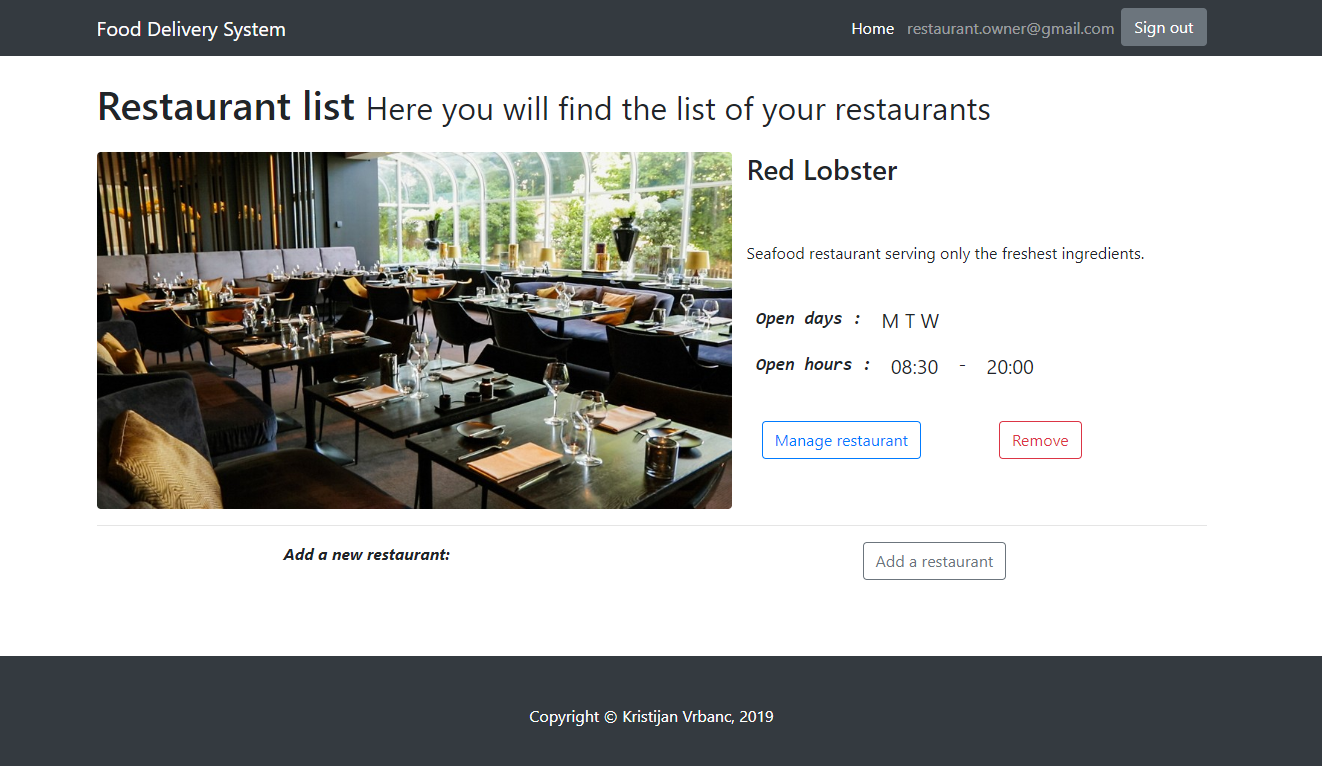
\includegraphics[height=7.8cm]{myrestaurants.png}
\caption{Stranica za pregled vlastitih restorana}
\label{fig:myRest}
\end{figure}

Također, stranica omogućava dodavanje novog restorana u sustav korištenjem obrasca prikazanog na slici 2.22. Sva polja obrasca su obavezna. Potrebno je unijeti naziv restorana, označiti dane u tjednu tijekom kojih je restoran otvoren, kratko opisati restoran, zadati njegovu lokaciju te učitati sliku koja će predstavljati taj restoran. Lokaciju restorana moguće je unijeti na dva načina. Prvi način je unosom adrese u polje \emph{location} i pritiskom na gumb \emph{Check the address} koji postavlja oznaku na kartu. Drugi način je postavljanjem oznake na kartu, čime se automatski postavlja pripadajuća adresa u polje \emph{location} što služi kao dodatna provjera prilikom unosa.
\begin{figure}[htb]
\centering
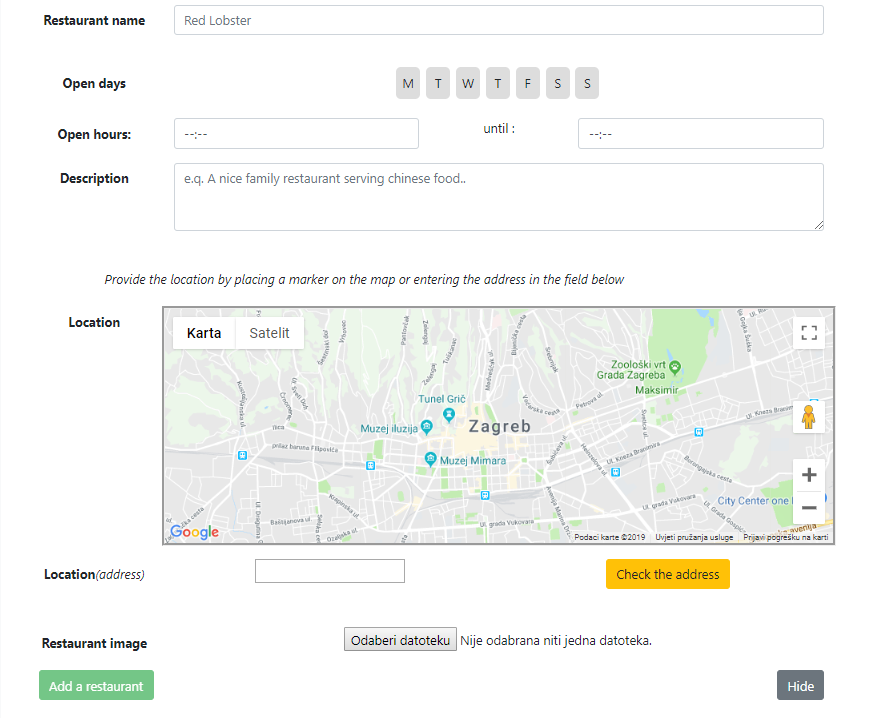
\includegraphics[height=8.0cm]{restoranObrazac.png}
\caption{Obrazac za dodavanje restorana u sustav}
\label{fig:obrRest}
\end{figure}
%----------------------------------------------------------------------------------------------------------------------------------------------------------
\subsection{Pregled jelovnika}
Stranica za pregled jelovnika dostupna je svim korisnicima osim korisicima sa ulogom dostavljača. Pogled na stranicu ovisi o ulozi korisnika u sustavu. 

Slika 2.23 prikazuje pogled neprijavljenog korisnika te korisnika sa ulogom kupca. Prikazan je kratki opis restorana koji sadži njegovo ime, radno vijeme te dani u tjednu tijekom kojih je restoran otvoren. Također, prikazana je slika restorana te njegova lokacija korištenjem usluge Google Maps. Korisniku je prikazan popis prehrambenih proizvoda restorana. Svaki prehrambeni proizvod prikazan je slikom, nazivom, opisom te jedniničnom cijenom u hrvatskim kunama. Korisniku sa ulogom kupca omogućeno je dodavanje proizvoda u košaricu uz naznaku količine korištenjem poveznice \emph{Add to cart}. Ukoliko se proizvod već nalazi u košarici, ispisuje se pripadna poruka. Neprijavljenom korisniku onemogućeno je dodavanje proizvoda u košaricu uz ispis pripadne poruke.
\begin{figure}[htb]
\centering
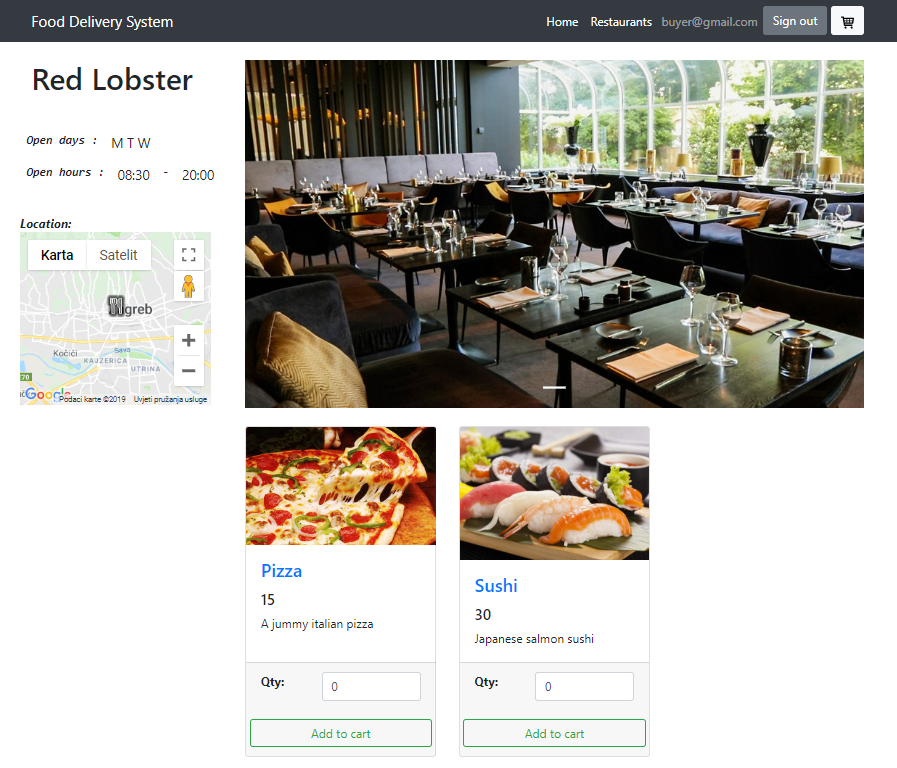
\includegraphics[height=8.7cm]{jelovnik.png}
\caption{Pogled neprijavljenog korisnika te kupca na stranicu za pregled jelovnika}
\label{fig:rrRest}
\end{figure}

Slika 2.24 prikazuje pogled korisnika sa ulogom vlasnika resotrana. Pogled dijeli elemente pogleda neprijavljenog korisnika i kupca, uz neke razlike. Korisniku nije prikazana lokacija već popis dostavljača koje je pridjelio tom restoranu. Također, omogućeno mu je dodavanje novih dostavljača u sustav putem obrasca. Dodavanje novog dostavljača iziskuje unos jedinstvene email adrese i odabir poveznice \emph{Add worker}. Ukoliko je dostavljač uspješno dodan, vlasniku se prikazuje email adresa te pripadna lozinka dostavljača koja je automatski generirana. Pomoću tih podataka dostavljač ima mogućnost prijave u sustav. Ukoliko dostavljač nije uspješno dodan, vlasniku se ispisuje odgovarajuća poruka. Također, vlasnik ima mogućnost uklanjanja dostavljača iz sustava.
\begin{figure}[htb]
\centering
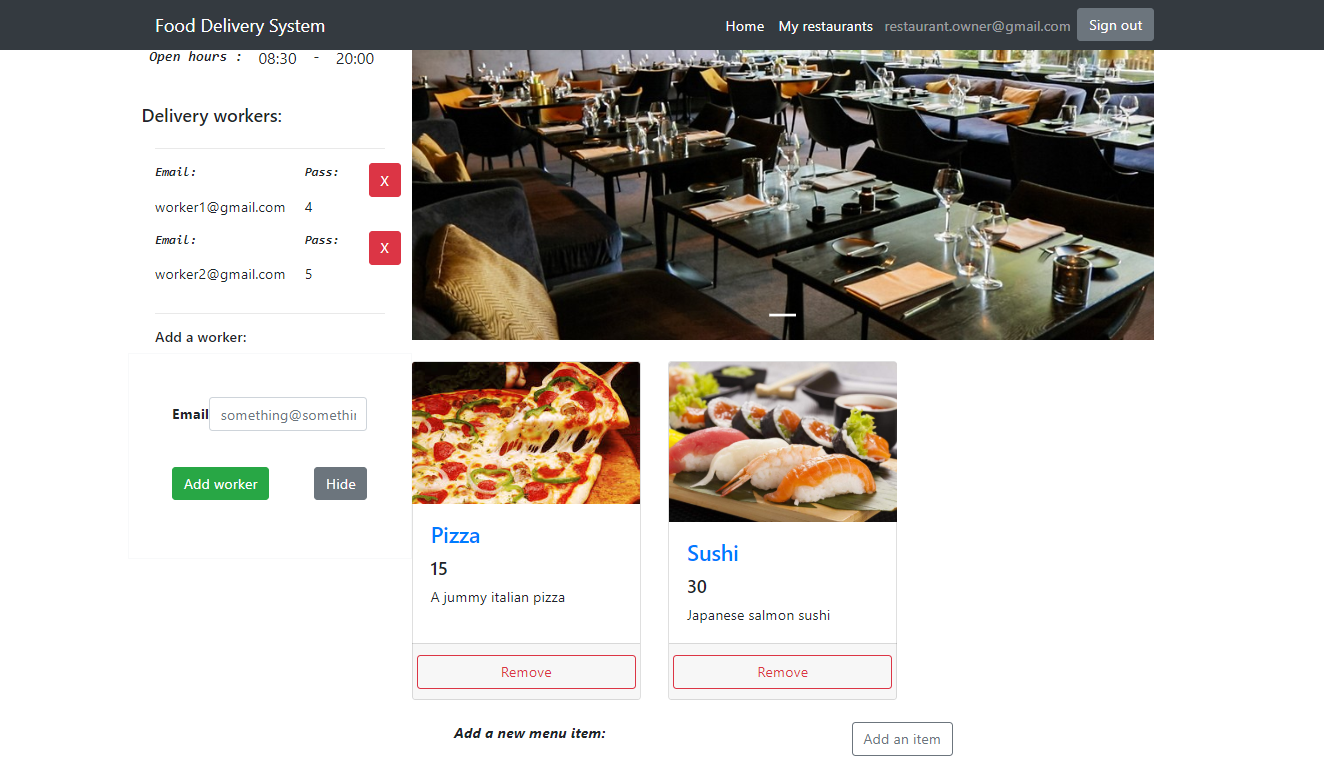
\includegraphics[height=8.5cm]{jelovnikVlasnik.png}
\caption{Pogled vlasnika restorana na stranicu za pregled jelovnika}
\label{fig:peerRest}
\end{figure}

Vlasnik također ima uvid u sve prehrambene proizvode prethodno dodane u sustav. za svaki proizvod, omogućeno mu je uklanjanje proizvoda iz sustava putem poveznice \emph{Remove}. Također, vlasnik je u mogućnosti dodavati nove proizvode u sustav putem obrasca na slici 2.25. Sva polja obrasca su obavezna. Obrazac zahtjeva unos imena proizvoda, opisa, jedinične cijene kao i slike koja će predstavljati proizvod.
\begin{figure}[htb]
\centering
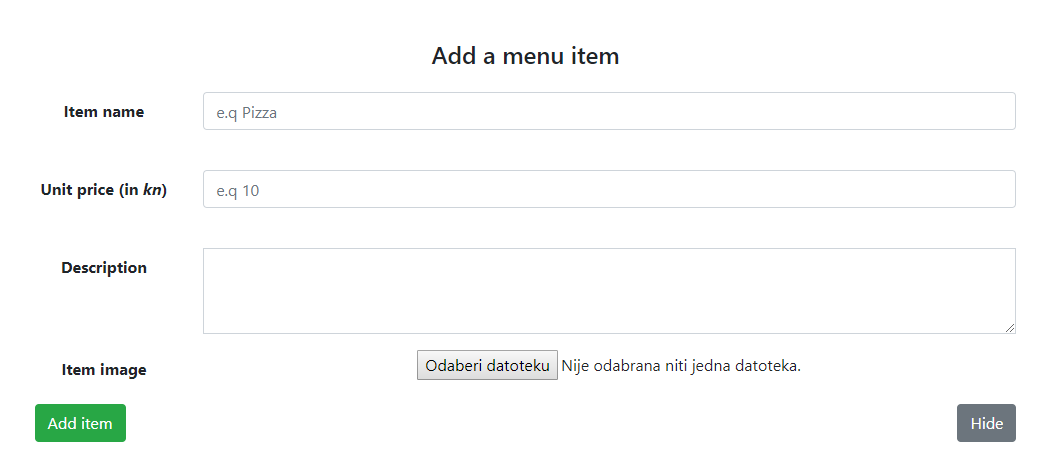
\includegraphics[height=6cm]{obrazacJelo.png}
\caption{Obrazac za dodavanje prehrambenog proizvoda u sustav}
\label{fig:obrJel}
\end{figure}  
%----------------------------------------------------------------------------------------------------------------------------------------------------------
\subsection{Košarica}
Prijavljenom korisniku sustava sa ulogom kupca omogućen je pregled virtualne košarice. U košarici se nalazi popis svih jela pripravnih za postavljanje narudžbe. Za svaki proizvod prikazana je slika tog proizvoda, naziv, jedinična cijena, postavljena količina te ukupna cijena proizvoda. Korisniku je omogućena promijena količine proizvoda postavljanjem polja količine te odabirom poveznice \emph{Change Qty.}. Također, kupcu je omogućeno uklanjanje proizvoda iz košarice.

Prilikom potvrde narudžbe, korisnik pruža lokaciju dostave. Lokacija se zadaje u polju iznad karte te pritiskom na gumb \emph{Check address} koja postavlja oznaku na kartu, ili postavljanjem oznake na kartu koja odgovarajuću adresu postavlja u polje adrese. Slika 2.26 prikazuje stranicu virtualne košarice.
\begin{figure}[htb]
\centering
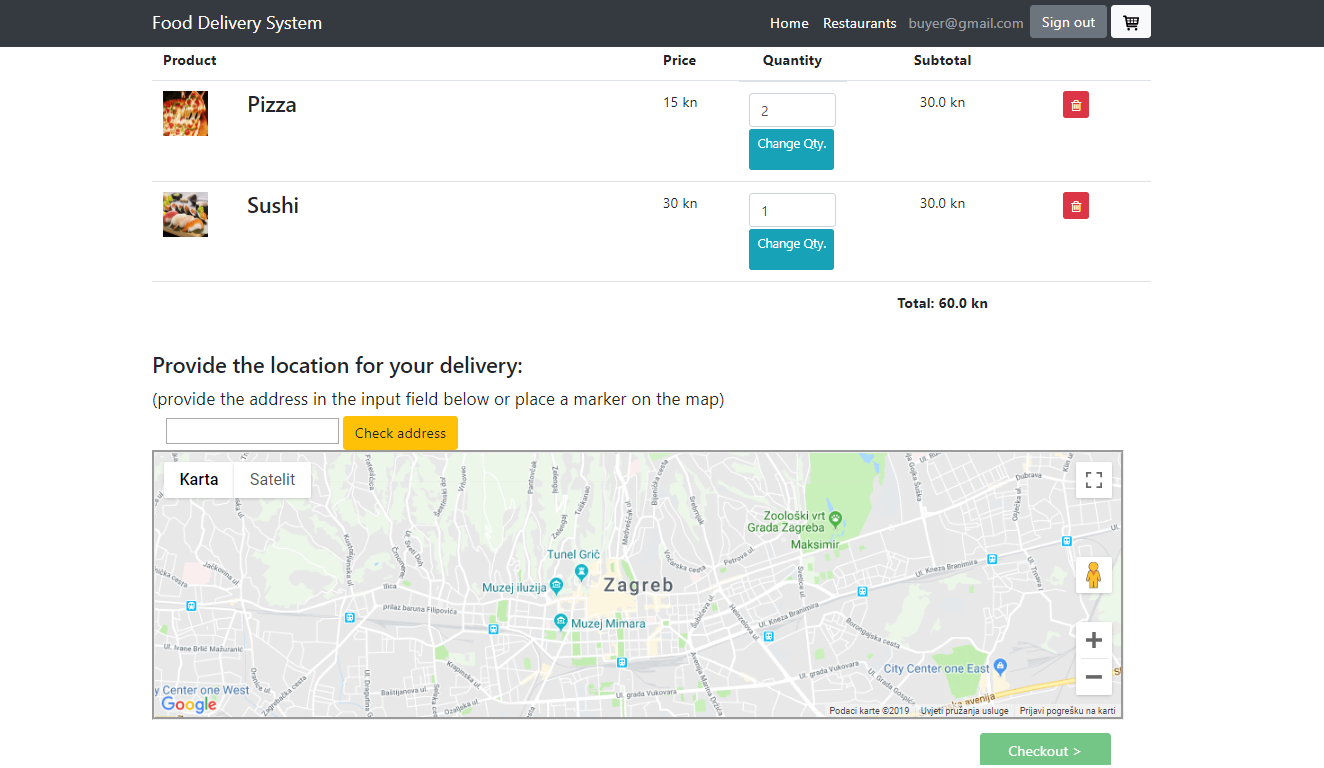
\includegraphics[height=8.5cm]{kosarica.png}
\caption{Stranica virtualne košarice}
\label{fig:kos}
\end{figure}  
%----------------------------------------------------------------------------------------------------------------------------------------------------------
\subsection{Pregled narudžba}
Pregled narudžba restorana omogućen je korisniku sa ulogom dostavljača hrane. Stranica koja se nalazi na slici 2.27 prikazuje popis svih nepreuzetih narudžba restorana za kojeg je dostavljač nadležan. Za svaku narudžbu, prikazan je broj narudžbe, korisničko ime osobe koja je podnijela narudžbu, količina naručenih proizvoda te ukupna cijena narudžbe. Korisniku je omogućeno preuzimanje dostave poveznicom \emph{Take order} nakon ćega se narudžba uklanja sa popisa.
\begin{figure}[htb]
\centering
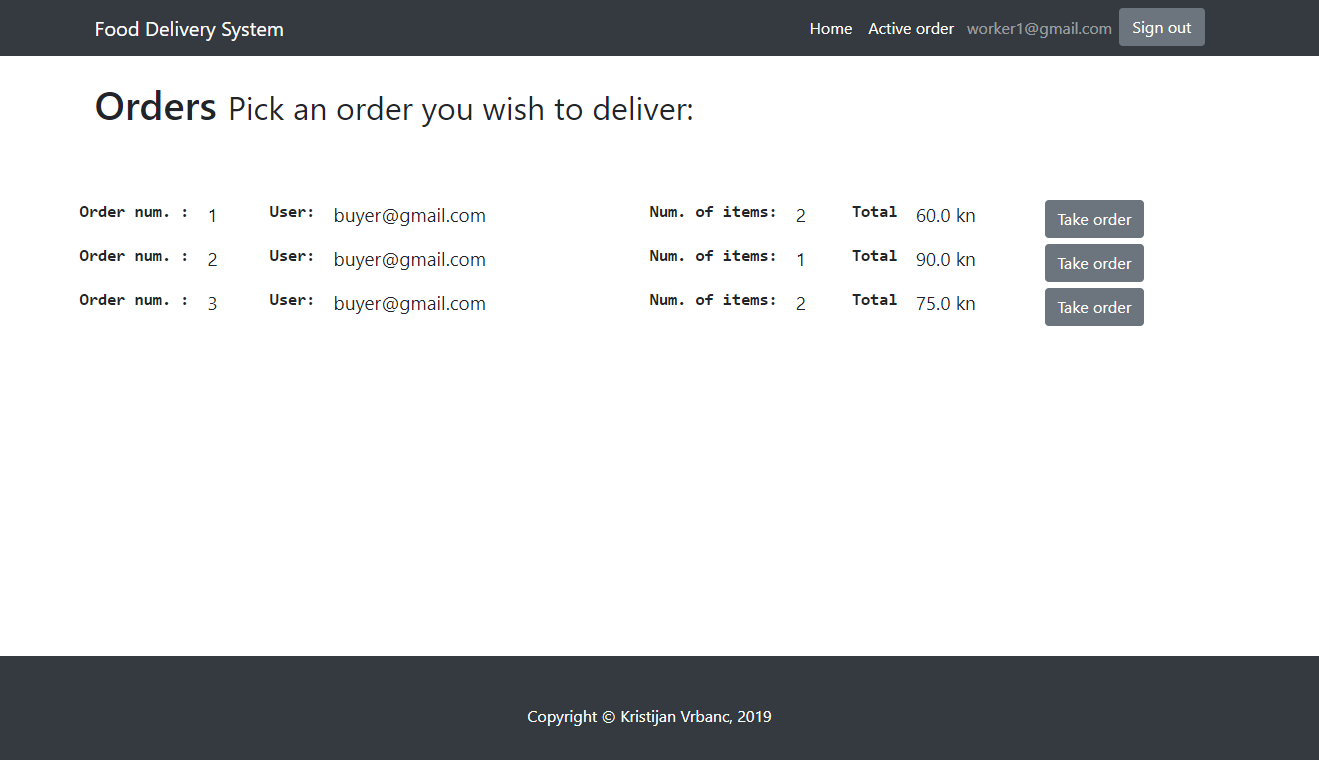
\includegraphics[height=7.8cm]{narudzbe.png}
\caption{Stranica za pregled narudžba}
\label{fig:nar}
\end{figure}
%----------------------------------------------------------------------------------------------------------------------------------------------------------
\subsection{Aktivna dostava}
Stranica aktivne dostave, prikazana na slici 2.28, omogućena je korisniku sa ulogom dostavljača hrane. Ukoliko je korisnik preuzeo dostavu neke narudžbe, prikazuju mu se svi podaci bitni za dostavu.
\begin{figure}[htb]
\centering
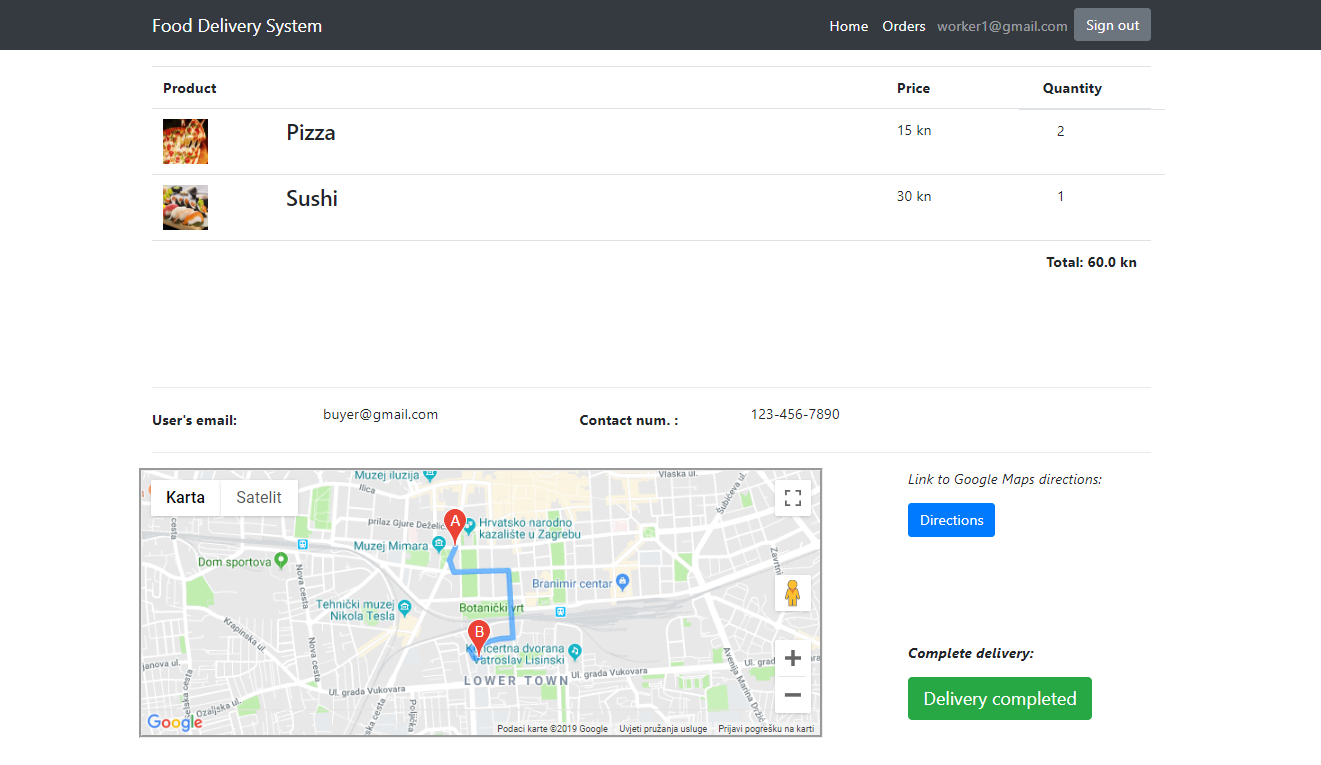
\includegraphics[height=8.0cm]{aktivna.png}
\caption{Stranica aktivne dostave}
\label{fig:nar}
\end{figure}

Prikazan je popis proizvoda koje je potrebno dotaviti, njihova jedinična cijena, količina i ukupna cijena. Također, dostavljaču je prikazano korisničko ime korisnika koji je podnio narudžbu, kao i korisnikov kontakt broj. Dostavljač na uvid dobiva kartu sa ucrtanim putem od restorana do lokacije koje je korisnik postavio za dostavu. Ukoliko dostavljač pristupa stranici preko pametnog telefona, poveznica \emph{Directions} otvara aplikaciju usluge Google Maps sa prikazom smjernica od restorana do  tražene lokacije.

Korištenjem  poveznice \emph{Delivery completed} korisnik završava dostavu.
%----------------------------------------------------------------------------------------------------------------------------------------------------------
\chapter{Zaključak}
Izrada web aplikacije zahtjevan je zadatak. Prije samog početka izrade potrebno je njeno dobro planiranje. Potrebno je definirati sve funkcionalne zahtjeve koje bi korisnici mogli imati na aplikaciju jer se tako mogu otkriti potencijalni problemi izrade. Također, na temelju funkcionalnih zahtjeva moguće je sagraditi rani koncept aplikacije koji se koristi prilikom izbora tehnologija za razvoj. 

Izbor razvojnih tehnologija također je vrlo važan proces. Dobar izbor tehnologija može uvelike olakšati izradu aplikacije. Potrebno je izabrati tehnologije koje pružaju mnogo funkcionalnosti. U kontekstu poslužiteljskih tehnologija to su funkcionalnosti poput sigurnosti aplikacije, pristupa bazi podataka, jednostavnog načina posluživanja korisničkih zahtjeva\ldots Kod klijentskih tehnologija potrebno je izabrati tehnologije koje pružaju veliku količinu gotovog koda, ali i jednostavan i intuitivan način za prilagođavanje tih gotovih dizajna i stvaranja svojih. Također, bitno je da tehnologije imaju što veću aktivnu zajednicu korisnika koji bi mogli pomoći pri učenju tehnologija te samoj izradi aplikacije.

Organizacija koda tadođer je jako bitna. Kod je potrebno organizirati u razrede i tematske pakete jer se time dobiva na modularnosti koda te lakše dodavaju novi dijelovi aplikacije i prepravljaju postojeći.

Naposljetku, kao zadnju fazu izrade aplikacije potrebo je provesti testiranje. Prolaze se sve zahtjevane funkcionalnosti korisnika te se isprobavaju svi mogući scenrariji korištenja aplikacije od strane korisnika. Testiranje služi kako bi se ispravili nedostaci u kodu, a samim time i povećalo zadovoljstvo korisnika.\\

Imajući sve to u vidu, možemo ustanoviti da izrada web aplikacije nije lak zadatak. Izrada se sastoji od mnogo faza koje iziskuju puno proučavanja, učenja, prilagođavanja ali i maštovitosti.

\bibliography{reference}
\bibliographystyle{fer}

\begin{sazetak}
Cilj ovoga rada je izrada web aplikacije. Sustav za dostavu hrane internet je trgovina gdje korisnici na lak i intuitivan način vrše pregled jelovnika i postavljaju narudžbe.  Rad opisuje odabrane tehnologije upotrijebljene pri razvoju aplikacije, kao i samu strukturu aplikacije te njenu funkcionalnost .

Odabrane razvojne tehnologije dijele se na klijentske i poslužiteljske. Klijentske tehnologije služe za definiranje sučelja prema korisniku, svega što korisnik vidi i sa čime može imati interakciju. Korištene klijentske tehnologije su HTML, CSS, JavaScript te razvoji okvir Bootstrap. Poslužiteljske tehnologije služe za obradu podataka generiranih od strane korisnika. Korištene poslužiteljske tehnologije su Thymeleaf te razvojni okvir Spring. Konkretno, korištena su četiri modula razvojnog okvira Spring: Spring Boot, Spring Security, Spring MVC te Spring Data JPA. Za komunikaciju sa bazom podataka korišten je jezik SQL.

Aplikacija podržava četiri tipa korisnika. Pogled korisnika na aplikaciju ovisi o njegovoj ulozi u sustavu.


\kljucnerijeci{web aplikacija, restoran, hrana, narudžba, dostava, smjernice, razvojni okvir Spring, Bootstrap}
\end{sazetak}

% TODO: Navedite naslov na engleskom jeziku.
\engtitle{Food delivery system}
\begin{abstract}
The aim of this paper is to create a web application. The food delivery system is a web shop that delivers an easier and more intuitive way to browse menus and place orders. The paper describes the selected technologies used in the development of the application, as well as the very structure of the application and its functionality.

Selected development technologies are devided into client and server technologies. Client technologies are used to define user interface, all that user sees and can interact. The client technologies used are HTML, CSS, JavaScript and Bootstrap framework. Server technologies are used to process data generated by users. The server technologies used are Thymeleaf and the Spring framework. Specifically, four of the Spring framework modules used are: Spring Boot, Spring Security, Spring MVC and Spring Data JPA. The SQL language was used to communicate with the database.

The application supports four types of users. The user's view of the application depends on his role in the system.

\keywords{web aplication, restaurant, food, order, delivery, directions, Spring framework, Bootstrap}
\end{abstract}

\end{document}
